% -------------------
% --- Definicia zakladnych pojmov
% --- Vyplnte podla vasho zadania
% -------------------
\def\mfrok{2016}
\def\mfnazov{Design and implementation of an RFID access control system}
\def\mftyp{Bachelor's Thesis}
\def\mfautor{Kamila Součková}
\def\mfskolitel{RNDr. Richard Ostertág, PhD. }

%ak mate konzultanta, odkomentujte aj jeho meno na titulnom liste
%\def\mfkonzultant{tit. Meno Priezvisko, tit. }

\def\mfmiesto{Bratislava, \mfrok}

%aj cislo odboru je povinne a je podla studijneho odboru autora prace
\def\mfodbor{2508 Informatics}
\def\program{ Informatics }
\def\mfpracovisko{ Department of Computer Science }

% -------------------
% --- Obalka ------
% -------------------
\thispagestyle{empty}

\begin{center}
\sc\large
Comenius University in Bratislava\\
Faculty of Mathematics, Physics and Informatics

\vfill

{\LARGE\mfnazov}\\
\mftyp
\end{center}

\vfill

{\sc\large
\noindent \mfrok\\
\mfautor
}

\eject % EOP i
% --- koniec obalky ----

% -------------------
% --- Titulný list
% -------------------

\thispagestyle{empty}
\noindent

\begin{center}
\sc
\large
Comenius University in Bratislava\\
Faculty of Mathematics, Physics and Informatics

\vfill

{\LARGE\mfnazov}\\
\mftyp
\end{center}

\vfill

\noindent
\begin{tabular}{ll}
Študijný program: & \program \\
Študijný odbor: & \mfodbor \\
Školiace pracovisko: & \mfpracovisko \\
Školiteľ: & \mfskolitel \\
% Konzultant: & \mfkonzultant \\
\end{tabular}

\vfill


\noindent \mfmiesto\\
\mfautor

\eject % EOP i


% --- Koniec titulnej strany


% -------------------
% --- Zadanie z AIS
% -------------------
% v tlačenej verzii s podpismi zainteresovaných osôb.
% v elektronickej verzii sa zverejňuje zadanie bez podpisov

\newpage
\thispagestyle{empty}
\hspace{-2cm}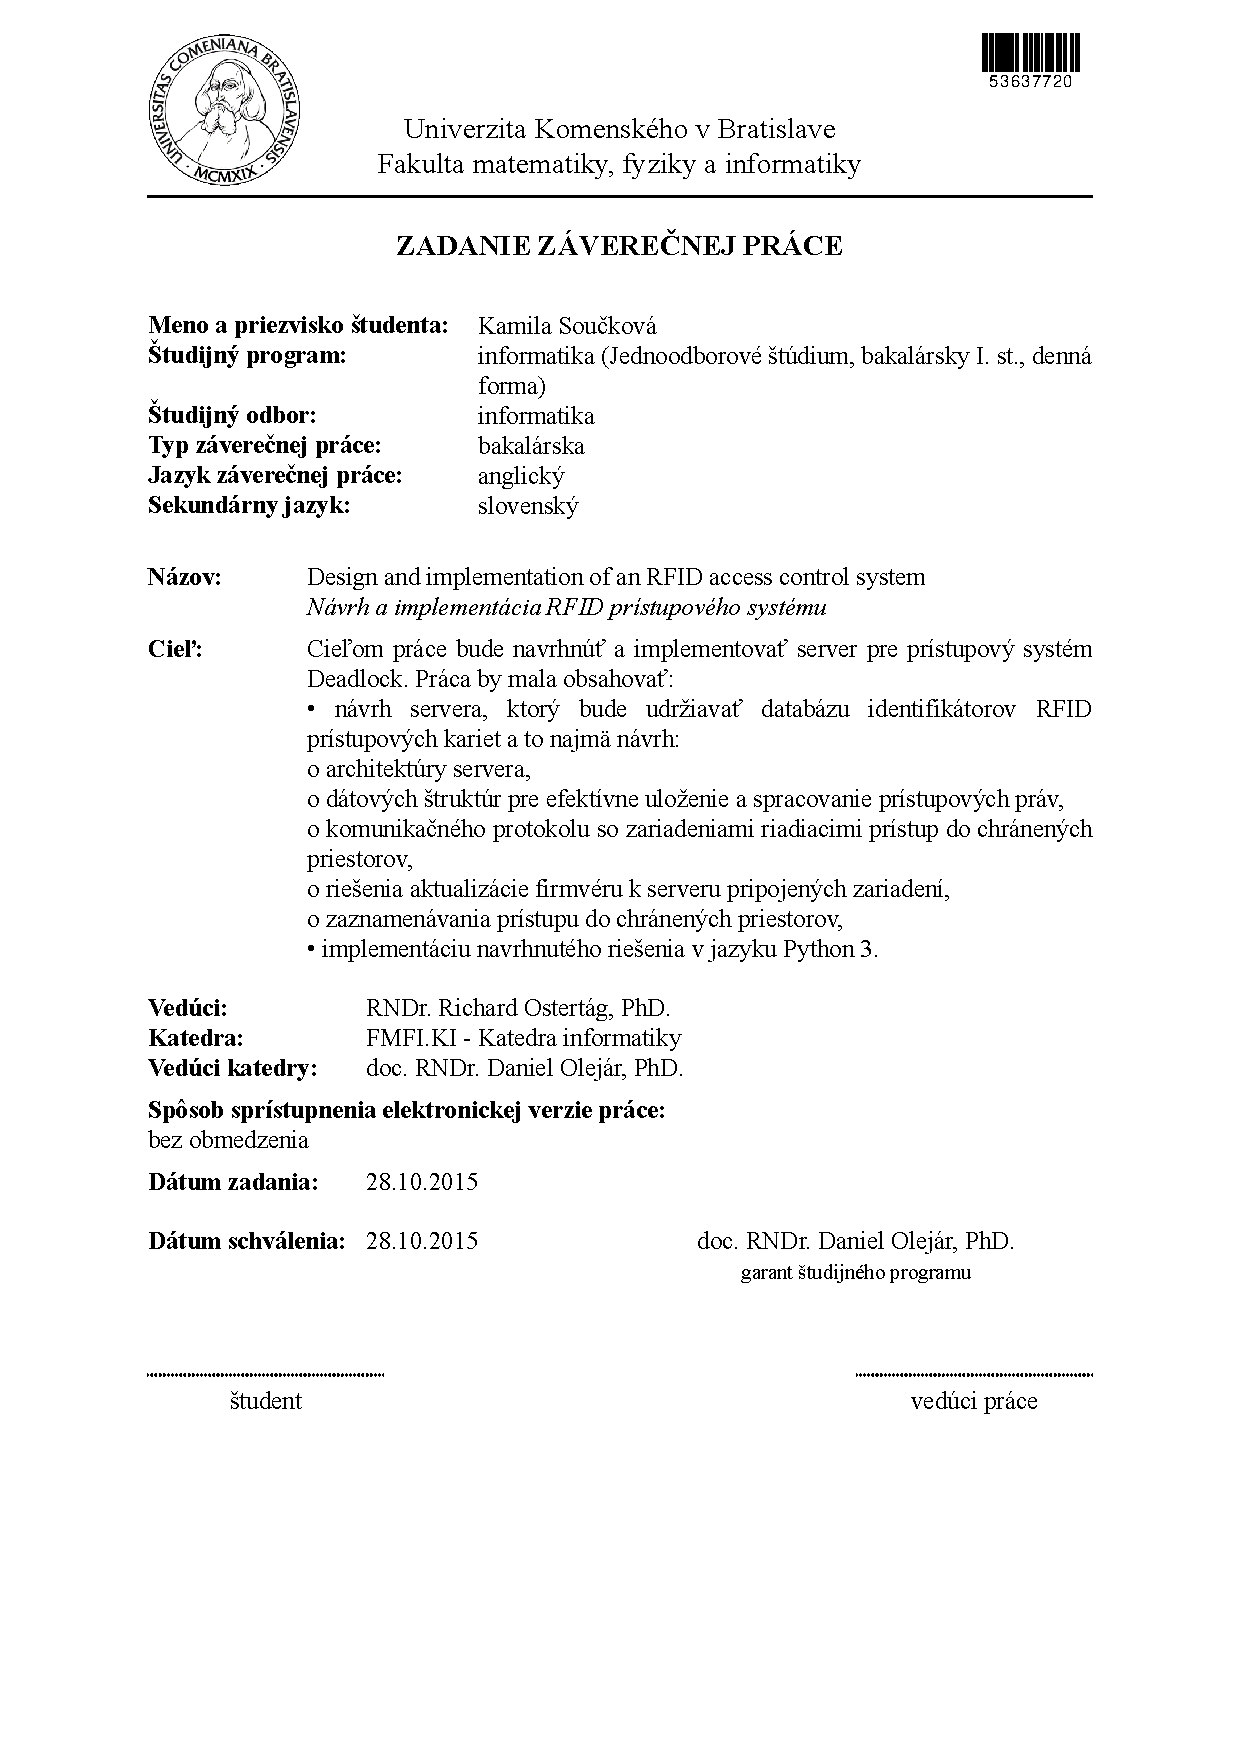
\includegraphics[width=1.1\textwidth]{src/img/zadanie}

% --- Koniec zadania

\frontmatter

% -------------------
%   Poďakovanie - nepovinné
% -------------------
\setcounter{page}{3}
\newpage
~

\vfill
\noindent\textbf{Acknowledgements:} \TODO{Jerry, Ostertág, Vinko, ŠVT/Adam, F za reviews?}

% --- Koniec poďakovania

% -------------------
% --- Abstrakt - Anglicky
% -------------------
\newpage
\section*{Abstract}

Abstract in the English language (translation of the abstract in the
Slovak language).


\paragraph*{Keywords:}

% --- Koniec Abstrakt - Anglicky

% -------------------
%   Abstrakt - Slovensky
% -------------------
\newpage
\section*{Abstrakt}


Slovenský abstrakt v rozsahu 100-500 slov, jeden odstavec. Abstrakt
stručne sumarizuje výsledky práce. Mal by byť pochopiteľný pre bežného
informatika. Nemal by teda využívať skratky, termíny alebo označenie
zavedené v práci, okrem tých, ktoré sú všeobecne známe.

\paragraph*{Kľúčové slová:} jedno, druhé, tretie (prípadne štvrté, piate)
% --- Koniec Abstrakt - Slovensky


% -------------------
% --- Predhovor - v informatike sa zvacsa nepouziva
% -------------------
%\newpage
%\thispagestyle{empty}
%
%\huge{Predhovor}
%\normalsize
%\newline
%Predhovor je všeobecná informácia o práci, obsahuje hlavnú charakteristiku práce
%a okolnosti jej vzniku. Autor zdôvodní výber témy, stručne informuje o cieľoch
%a význame práce, spomenie domáci a zahraničný kontext, komu je práca určená,
%použité metódy, stav poznania; autor stručne charakterizuje svoj prístup a svoje
%hľadisko.
%
% --- Koniec Predhovor


% -------------------
% --- Obsah
% -------------------

\newpage

\tableofcontents

% ---  Koniec Obsahu

% -------------------
% --- Zoznamy tabuliek, obrázkov - nepovinne
% -------------------

%\newpage

%\listoffigures

% ---  Koniec Zoznamov

\mainmatter
